\subsection{Lab15: Transmisor AM}

%*********************
\begin{frame}{}

\pgfdeclareimage[width=\paperwidth,height=\paperheight]{bg}{imagenes/fondo_lab}
\setbeamertemplate{background}{\pgfuseimage{bg}}

\bfseries{\textrm{\LARGE Lab15\\ \Large Transmisor AM}}
\raggedright
\end{frame}
%*********************

\begin{frame}{La Modulación de Amplitud IQ}

\pgfdeclareimage[width=\paperwidth,height=\paperheight]{bg}{imagenes/fondo3}
\setbeamertemplate{background}{\pgfuseimage{bg}}

Es una modulación digital en la que la señal moduladora (información) está contenido tanto en la amplitud como en la fase de la señal transmitida, se transmite dos mensajes independientes por un único canal, esto se consigue modulando una misma portadora, desfasada 90$^{\circ}$ de la señal moduladora formando dos canales ortogonales en el mismo ancho de banda, con lo cual se mejora en eficiencia de ancho de banda.\\
\vspace{2mm}
La modulación AM está conformada por dos canales i(t) y q(t), el canal i(t) es la señal moduladora que contiene la información y es la parte real para la transmisión, el canal q(t) es la señal portadora que debe estar desfasada 90$^{\circ}$ de la señal moduladora y es la parte imaginaria para la transmisión.

\begin{figure}[H]
%\centering
\vspace{-3mm}
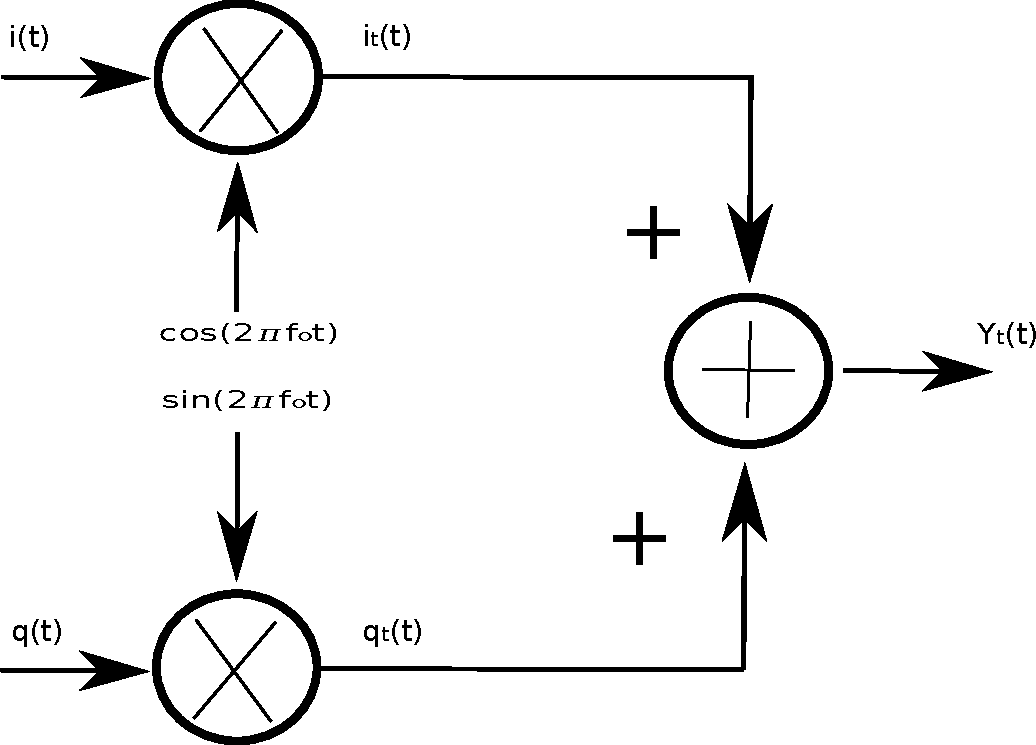
\includegraphics[width=.5\textwidth]{parte3/lab15/pdf/lab15_1.pdf}
\end{figure}

\end{frame}
%---------------------------------

\begin{frame}{La Modulación de Amplitud IQ}

Matemáticamente se expresa: \\\vspace{3mm}
\centering{
$i_t (t)=i(t)cos(2\pi f_0 t + 0^{\circ})$ \\ \vspace{2mm}
$q_t (t)=q(t)cos(2\pi f_0 t + 90^{\circ})=q(t)sin(2\pi f_0 t)$\\ \vspace{2mm}
$y_t (t)= \sqrt{i^{2} (t)+q^{2}(t)}cos(2\pi f_0 t + \theta(t))$}\\ \vspace{2mm}
$\theta(t)=tan^{-1}\frac{q(t)}{i(t)}$\\\vspace{2mm}
$-180<\theta<180^{\circ}$

\end{frame}
%---------------------------------


\begin{frame}{La Modulación de Amplitud IQ}

\begin{figure}[H]
\centering
\vspace{-3mm}
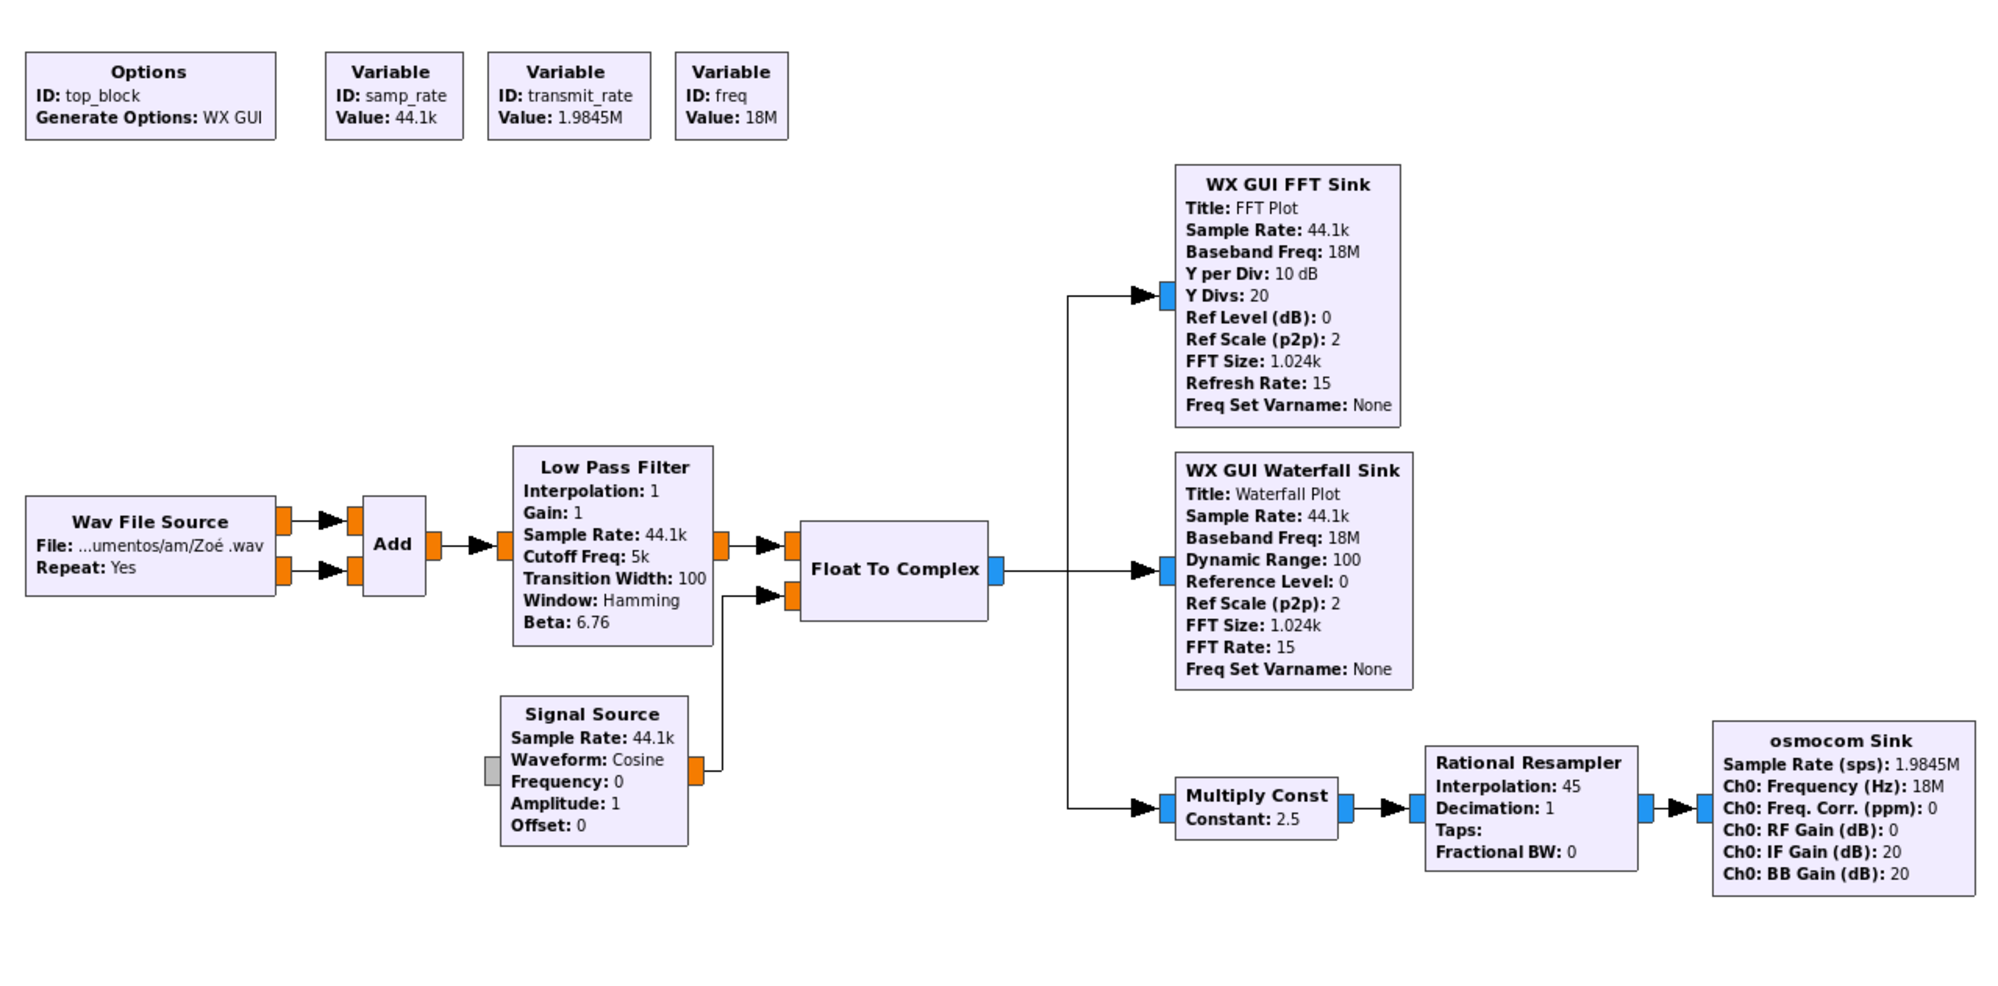
\includegraphics[width=\textwidth]{parte3/lab15/pdf/lab15_2.pdf}
\end{figure}

\end{frame}
%---------------------------------

\begin{frame}{La Modulación de Amplitud IQ}

\begin{figure}[H]
\centering
\vspace{-3mm}
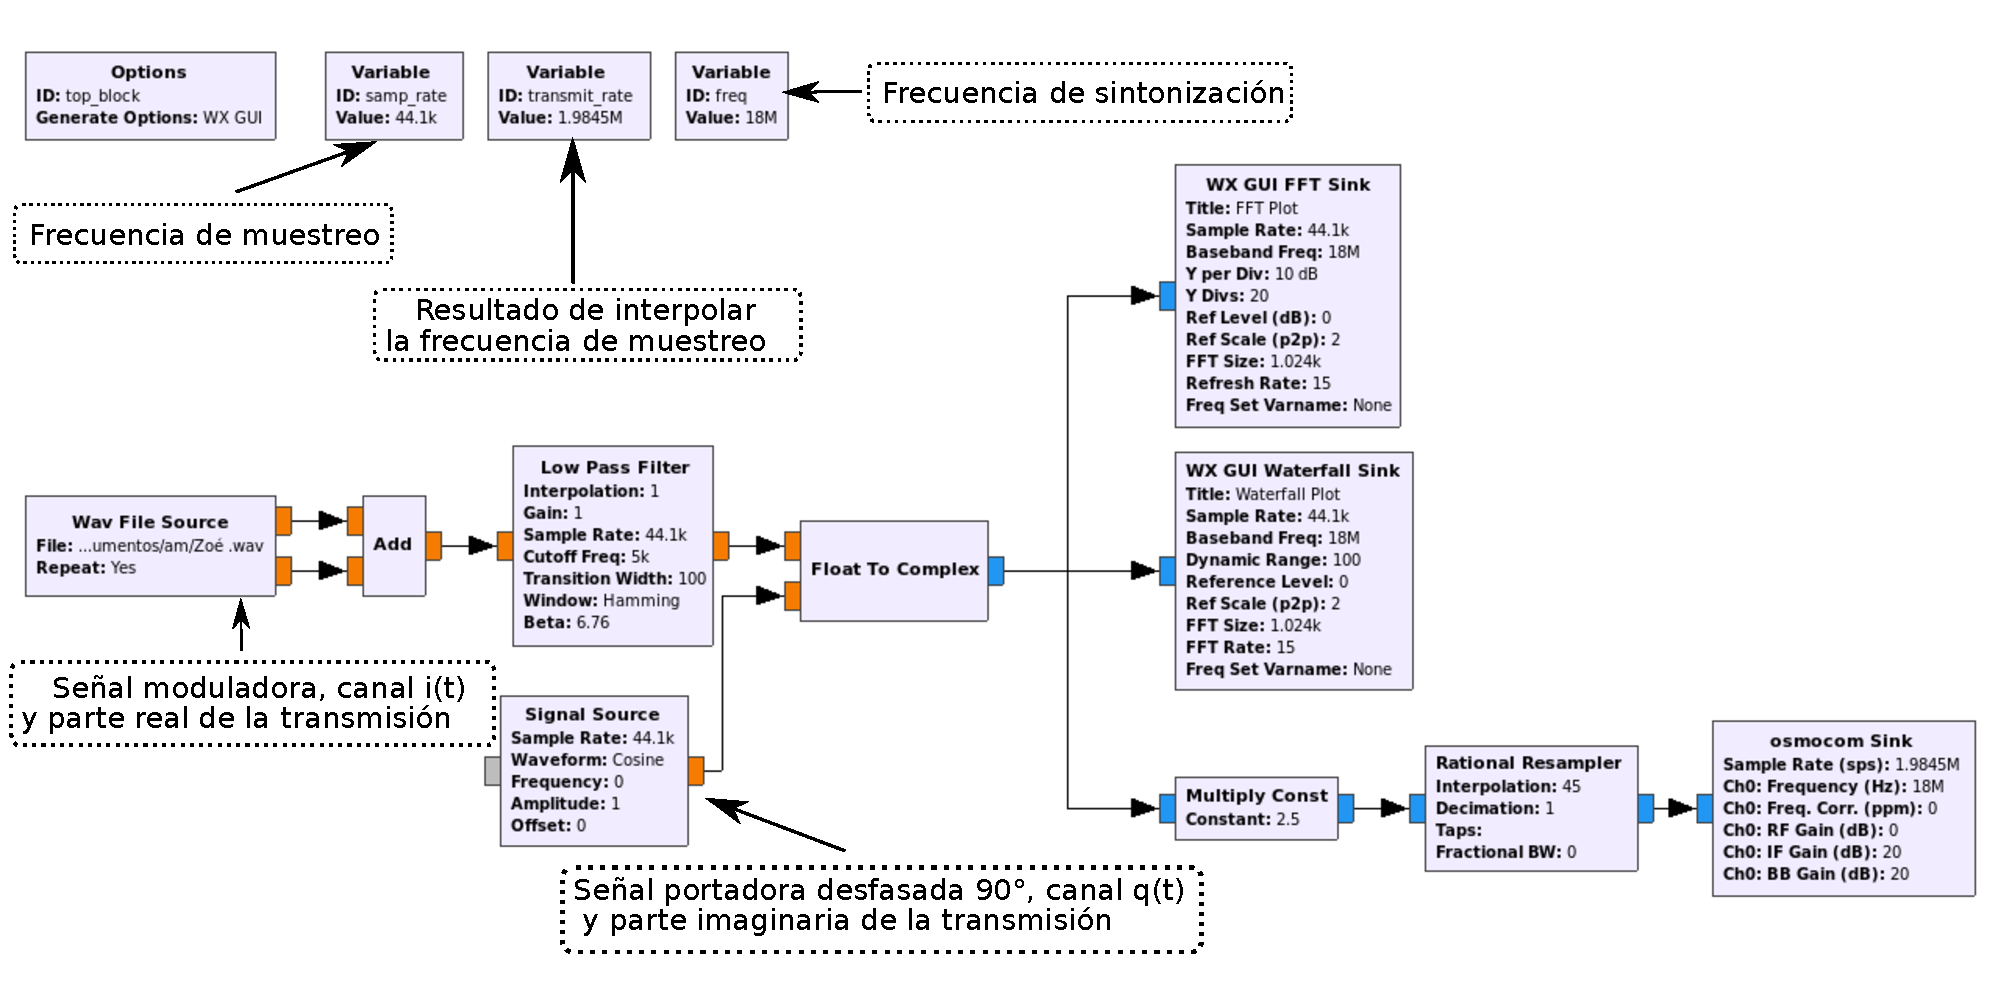
\includegraphics[width=\textwidth]{parte3/lab15/pdf/lab15_3.pdf}
\end{figure}

\end{frame}
%---------------------------------

\begin{frame}{La Modulación de Amplitud IQ}


El resultado de la modulación (señal modulada) no se puede observar en el dominio del tiempo ni de la frecuencia ya que el proceso de mezclado entre la señal portadora y moduladora se hace directamente con el software es decir en la Hack, pero si se puede observar el resultado de la unión entre la parte real e imaginaria (señal moduladora y portadora).  La frecuencia utilizada para mirar la señal en el dominio de la frecuencia (FFT) y el diagrama de cascada (espectrograma) es la sintonizada en el radio.

\end{frame}
%---------------------------------

\begin{frame}{Resultado}

\begin{figure}[H]
\centering
\vspace{-3mm}
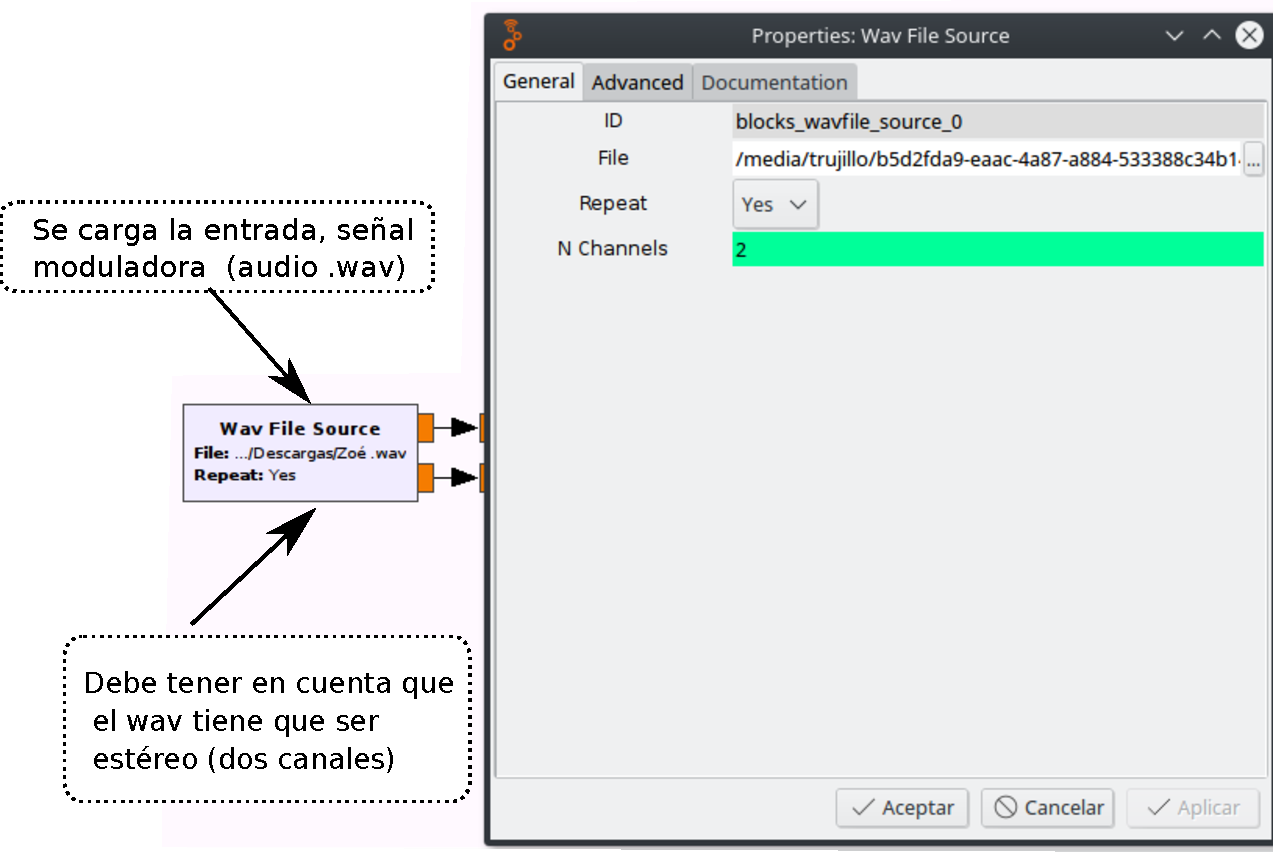
\includegraphics[width=\textwidth]{parte3/lab15/pdf/lab15_4.pdf}
\end{figure}

\end{frame}
%---------------------------------